\documentclass[tikz,border=10pt]{standalone}
\usepackage{tikz}
\usepackage{verbatim}
\begin{document}

\tikzset{every picture/.style={line width=0.75pt}} %set default line width to 0.75pt

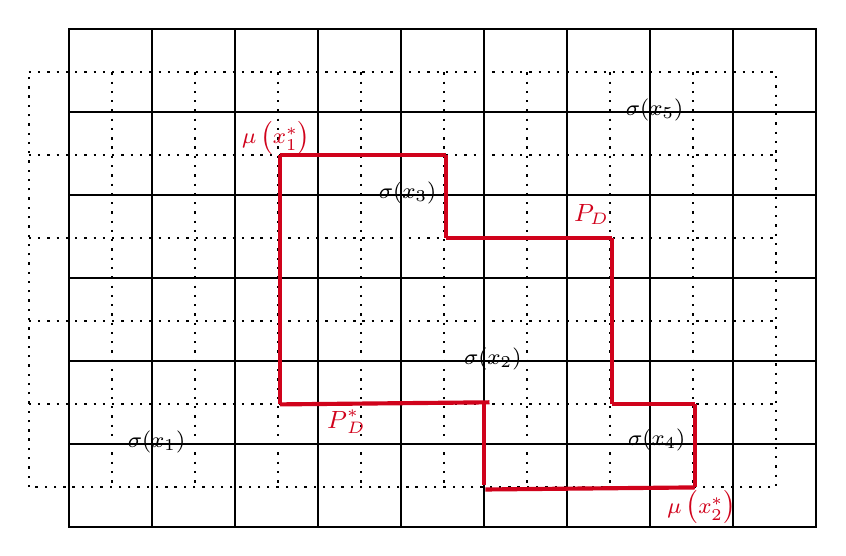
\begin{tikzpicture}[x=0.75pt,y=0.75pt,yscale=-1,xscale=1]
%uncomment if require: \path (0,300); %set diagram left start at 0, and has height of 300

%Shape: Grid [id:dp34601834790467834]
\draw  [draw opacity=0][line width=0.75]  (95,21) -- (455,21) -- (455,261) -- (95,261) -- cycle ; \draw  [line width=0.75]  (135,21) -- (135,261)(175,21) -- (175,261)(215,21) -- (215,261)(255,21) -- (255,261)(295,21) -- (295,261)(335,21) -- (335,261)(375,21) -- (375,261)(415,21) -- (415,261) ; \draw  [line width=0.75]  (95,61) -- (455,61)(95,101) -- (455,101)(95,141) -- (455,141)(95,181) -- (455,181)(95,221) -- (455,221) ; \draw  [line width=0.75]  (95,21) -- (455,21) -- (455,261) -- (95,261) -- cycle ;
%Shape: Grid [id:dp6443386042081738]
\draw  [draw opacity=0][dash pattern={on 0.84pt off 2.51pt}][line width=0.75]  (75.5,42) -- (435.5,42) -- (435.5,242) -- (75.5,242) -- cycle ; \draw  [dash pattern={on 0.84pt off 2.51pt}][line width=0.75]  (115.5,42) -- (115.5,242)(155.5,42) -- (155.5,242)(195.5,42) -- (195.5,242)(235.5,42) -- (235.5,242)(275.5,42) -- (275.5,242)(315.5,42) -- (315.5,242)(355.5,42) -- (355.5,242)(395.5,42) -- (395.5,242) ; \draw  [dash pattern={on 0.84pt off 2.51pt}][line width=0.75]  (75.5,82) -- (435.5,82)(75.5,122) -- (435.5,122)(75.5,162) -- (435.5,162)(75.5,202) -- (435.5,202) ; \draw  [dash pattern={on 0.84pt off 2.51pt}][line width=0.75]  (75.5,42) -- (435.5,42) -- (435.5,242) -- (75.5,242) -- cycle ;
%Straight Lines [id:da49630526944883124]
\draw [color={rgb, 255:red, 208; green, 2; blue, 27 }  ,draw opacity=1 ][line width=1.5]    (196.5,82) -- (276.5,82) ;
%Straight Lines [id:da9042395450781473]
\draw [color={rgb, 255:red, 208; green, 2; blue, 27 }  ,draw opacity=1 ][line width=1.5]    (276.5,122) -- (356.5,122) ;
%Straight Lines [id:da3551178432680273]
\draw [color={rgb, 255:red, 208; green, 2; blue, 27 }  ,draw opacity=1 ][line width=1.5]    (356.5,202) -- (356.5,122) ;
%Straight Lines [id:da28105816519272175]
\draw [color={rgb, 255:red, 208; green, 2; blue, 27 }  ,draw opacity=1 ][line width=1.5]    (276.5,82) -- (276.5,122) ;
%Straight Lines [id:da33861584446936677]
\draw [color={rgb, 255:red, 208; green, 2; blue, 27 }  ,draw opacity=1 ][line width=1.5]    (356.5,202) -- (396.5,202) ;
%Straight Lines [id:da8591992518763039]
\draw [color={rgb, 255:red, 208; green, 2; blue, 27 }  ,draw opacity=1 ][line width=1.5]    (396.5,202) -- (396.5,242) ;
%Straight Lines [id:da5572884320502969]
\draw [color={rgb, 255:red, 208; green, 2; blue, 27 }  ,draw opacity=1 ][line width=1.5]    (196.5,82) -- (196.5,202) ;
%Straight Lines [id:da4382771367852276]
\draw [color={rgb, 255:red, 208; green, 2; blue, 27 }  ,draw opacity=1 ][line width=1.5]    (196.5,202) -- (297.5,201) ;
%Straight Lines [id:da32264042537351045]
\draw [color={rgb, 255:red, 208; green, 2; blue, 27 }  ,draw opacity=1 ][line width=1.5]    (295,201) -- (295,241) ;
%Straight Lines [id:da7816067518401415]
\draw [color={rgb, 255:red, 208; green, 2; blue, 27 }  ,draw opacity=1 ][line width=1.5]    (295.5,243) -- (396.5,242) ;

% Text Node
\draw (177,64.4) node [anchor=north west][inner sep=0.75pt]  [font=\footnotesize,color={rgb, 255:red, 208; green, 2; blue, 27 }  ,opacity=1 ]  {$\mu \left( x_{1}^{*}\right)$};
% Text Node
\draw (382,242.4) node [anchor=north west][inner sep=0.75pt]  [font=\footnotesize,color={rgb, 255:red, 208; green, 2; blue, 27 }  ,opacity=1 ]  {$\mu \left( x_{2}^{*}\right)$};
% Text Node
\draw (122,213.4) node [anchor=north west][inner sep=0.75pt]  [font=\footnotesize,color={rgb, 255:red, 0; green, 0; blue, 0 }  ,opacity=1 ]  {$\sigma ( x_{1})$};
% Text Node
\draw (284,173.4) node [anchor=north west][inner sep=0.75pt]  [font=\footnotesize,color={rgb, 255:red, 0; green, 0; blue, 0 }  ,opacity=1 ]  {$\sigma ( x_{2})$};
% Text Node
\draw (243,93.4) node [anchor=north west][inner sep=0.75pt]  [font=\footnotesize,color={rgb, 255:red, 0; green, 0; blue, 0 }  ,opacity=1 ]  {$\sigma ( x_{3})$};
% Text Node
\draw (363,212.4) node [anchor=north west][inner sep=0.75pt]  [font=\footnotesize,color={rgb, 255:red, 0; green, 0; blue, 0 }  ,opacity=1 ]  {$\sigma ( x_{4})$};
% Text Node
\draw (362,53.4) node [anchor=north west][inner sep=0.75pt]  [font=\footnotesize,color={rgb, 255:red, 0; green, 0; blue, 0 }  ,opacity=1 ]  {$\sigma ( x_{5})$};
% Text Node
\draw (337,104.4) node [anchor=north west][inner sep=0.75pt]  [font=\small]  {$\textcolor[rgb]{0.82,0.01,0.11}{P_{D}}$};
% Text Node
\draw (218,203.4) node [anchor=north west][inner sep=0.75pt]  [font=\small]  {$\textcolor[rgb]{0.82,0.01,0.11}{P}\textcolor[rgb]{0.82,0.01,0.11}{_{D}^{*}}$};


\end{tikzpicture}
\end{document}
